\chapter{Configuration}\label{cha:configuration}\label{conf:configuration}
XCSoar is a highly configurable glide computer and can be customised
to suit a wide variety of preferences and user requirements.  This
chapter describes the configuration settings and options.

\section{Scope of configuration}

There are several ways XCSoar can be customised:
\begin{itemize}

\item Modifying configuration settings.  This is the sort of configuration
  most likely to be performed by users; and this is given the greatest attention 
  in this document.
\item Changing the language, or even just to change the wording
  of text in the user interface.
\item Changing the button assignments and button menus.  This allows 
  the content and structure of the button menu to be changed. 
\item Changing or adding actions performed when glide computer events
  take place.
\item Defining how long status messages appear and sounds to be played
  when those messages occur.
\end{itemize}
Describing all of these in a detail level like a reference manual would 
do is beyond the scope of this document. The user is referred to browse 
through the XCSoar Wiki for more details. 
\url{http://www.xcsoar.org/trac/wiki}

\section{Modifying settings}

There is a large set of configuration settings that may be customised
from the Settings dialogue accessible from the menu.
\menulabel{\bmenug{Config 2}\blink\bmenus{System}}
The configuration can be accessed through a two layer structured menu 
or just sequentially through the back and forward buttons.

\begin{center}
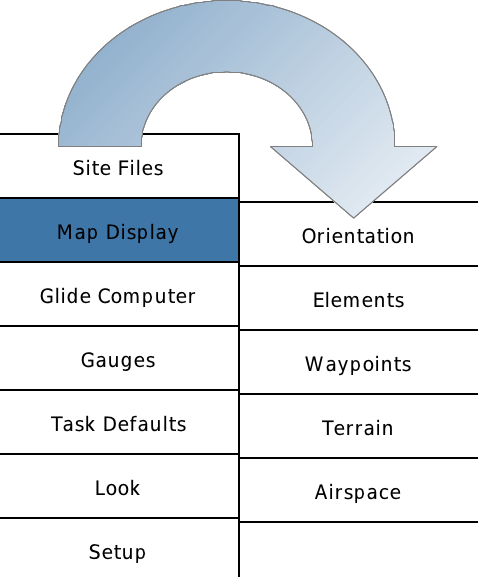
\includegraphics[angle=0,width=0.5\linewidth,keepaspectratio='true']{figures/config-menu.png}
\end{center}

You are strongly discouraged from changing these settings during
flight.  \warning  All changes to the settings should be performed on the ground
so that their desired effect on the programs behaviour can be
verified.

The settings dialogue contains several pages.  Once changes have been made,
click the Close button on the screen or PWR/ESC on Altair to close the dialogue
and return to the configuration menu. Another button press leads back to 
the normal map mode.

\tip Once you are happy with your configuration settings, save the
profile file and make a backup so that you can later restore the
settings if your PDA's memory is accidentally erased.

See Chapter~\ref{cha:data-files} for a description of the data formats
of files referred to in the settings.  Where no file is to be used,
the field can be left blank.  File name fields in forms show files
that match a file extension filter.  This makes it much easier to find
and select the correct file.

The main configuration dialogue (Setup System) can be run in Basic or
Expert user level, via a selectable field on the left of the dialogue.
\sketch{figures/config-expert.png}
When in Basic mode, many of the less commonly used and advanced
configuration settings are hidden.  In the descriptions below,
all of the parameters marked with an asterisk are only visible in
expert user level. 

%%%%%%%%%%%%%%%%%%
\section{Site Files / Site Files}
The dialogue specifies most of the important files that must be
configured when flying at a new site.

\begin{description}
\item[XCSoar data path]  The location for all of your XCSoar data on your hard drive, 
  SD card, or the PDA's static memory.
\item[Map Database]  The name of the map file (XCM) containing digital elevation
  terrain data, topography, and optionally waypoints, airspace etc. A good
  prepared database file covers all the needs for this page.
\item[Waypoints]  Primary waypoints file.  If left blank, waypoints are loaded
  from the map file (if available).
\item[More waypoints*]  Secondary waypoints file.  This may be used to add 
  waypoints for a competition.
\item[Watched waypoints*]  Waypoint file containing special waypoints for 
  which additional computations   like calculation of arrival height in map 
  display always takes place. Useful for waypoints   like known reliable 
  thermal sources (e.g. powerplants) or mountain passes.
\item[Airspaces]  The file name of the primary airspace file.  If left blank,
  airspaces are loaded from the map file (if available).
\item[More airspaces*]  The file name of the secondary airspace file.
\item[Waypoint details*]  The airfields file may contain extracts from 
  Enroute Supplements or other contributed information about individual airfields.
\end{description}

Airspace files define Special Use Airspace.  Up to two files may be
specified, the first for the main SUA file, and the second is intended
for use with NOTAM airspace, and is referred to as the additional
airspace file.
\sketch{figures/config-site.png}

The XCM map database concept is the current way to setup a site to fly.
XCSoar releases prior to v6.4 required each to be separate files and to be
specified separately (as the `{\it Terrain file}' and `{\it Topography file}' respectively). This 
option has been dropped in favor to the XCM map database with XCSoar release v6.4.  

The XCM map file, however, contains all these files: Terrain, topography
and optionally waypoints and airspaces.  If the latter are contained, the e.g. `{\it Primary waypoint file}' 
may be left blank and the system will load waypoints from the map file. 
However, the user can still specify other files and they will be used instead of 
the data in the map file.

See Section~\ref{sec:map} for more details on map files.


%%%%%%%%%%%%%%%%%%
\section{Map Display / Orientation}\label{sec:map-projection}

This page let you specify the favoured map orientation and view.

\begin{description}
\item[Cruise/Circling orientation]  \label{conf:orientation} This determines how
  the screen is rotated with the glider, depending on it's current display mode. \\
  {\bf Track up}: The moving map display will be rotated so the glider's track
  is oriented up. The north arrow symbol points to true north. The glider symbol 
  may be shown rotated according to the computed heading of the glider taking 
  wind into account. \\
  \sketch{figures/config-map_projection.png}
  {\bf Heading up}: The moving map display will be rotated so the glider's 
  heading is oriented up. \\
  {\bf North up}: The moving map display will always be orientated true north to
  south and the glider icon will be rotated to show its course (corrected for
  wind). \\
  {\bf Target up}: The moving map display will be rotated so the current target
  direction is oriented up. \\
  {\bf Wind up} The moving map display will be rotated so the wind is always 
  oriented top-down (might be useful for wave flying).
\item[Circling zoom]  \label{conf:circlingzoom} This determines whether separate
  zoom levels will be maintained for circling and cruise modes.  If enabled, then the 
  map will zoom in automatically when entering circling mode and zoom out
  automatically when leaving circling mode.
\item[Map shift reference]  The direction according to the map will be displaced 
  in order to present a meaningful map section. \\
  {\bf None}: Disable any adjustment. \\
  {\bf Track}: Use a recent average of the ground track as basis. \\
  {\bf Target}: Use the current target waypoint as basis.
\item[Glider position offset]  \label{conf:gliderposition} Defines the location of the 
  glider drawn on the screen in percent from the screen edge.
\item[Max. auto zoom distance]  The upper limit for auto zoom distance.
\end{description}


%%%%%%%%%%%%%%%%%%
\section{Map Display / Elements}\label{sec:map-elements}

This page provides options relating to screen elements overlayed to the map display.

\begin{description}
\item[Ground track]  Display the ground track (ground track projection) on the map.
  The setting "Auto" displays the ground track only if there is a significant 
  difference to plane heading.
\item[FLARM traffic]  \label{conf:flarm-on-map} This enables the display of FLARM 
  traffic on the map.
\item[Trail length*] \label{conf:snailtrail} Determines whether and how long a
  snail trail is drawn behind the glider. \\
\sketch{figures/config-map_elements.png}
  {\bf Off}: No trail is drawn. \\
  {\bf Long}: A long trail is drawn (approx 60 minutes). \\
  {\bf Short}: A short trail is drawn (approx 10 minutes). \\
  {\bf Full}: A trail for the entire flight is drawn.
\item[Trail drift*] \label{conf:traildrift} Determines whether the
  snail trail is drifted with the wind when displayed in circling mode.  Switched Off,
  the snail trail stays uncompensated for wind drift.
\item[Trail type*] \label{conf:snailtype} Sets the type of the snail trail display. \\
  {\bf Vario \#1}: Within lift areas lines get displayed green and
  thicker, while sinking lines are shown brown and thin.  Zero lift
  is presented as a grey line. \\
  {\bf Vario \#1 (with dots)}: The same colour scheme as the previous, but with dotted 
  lines while sinking. \\
  {\bf Vario \#2}: The climb colour for this scheme is orange to red, sinking is
  displayed as light blue to dark blue. Zero lift is presented as a yellow line. \\
  {\bf Vario \#2 (with dots)}: The same colour scheme as the previous, but with dotted 
  lines while sinking. \\
  {\bf Altitude}: The colour scheme corresponds to the altitude.
\item[Trail scaled*] \label{conf:trailscaled} If set to ON the snail trail 
  width is scaled according to the vario signal.
\item[Detour cost markers*]  If enabled this displays in cruise flight some
  figures projected in front of the nose of the glider icon.  This is the
  additional distance in percent if you fly up the position of the figure and
  after that again straight towards the target, compared to the straight distance
  to target.
\item[Aircraft symbol*]  Sets the symbol used for the aircraft. \\
  {\bf Simple}: Simplified line graphics, a black glider shape with white contours. \\
  {\bf Simple (large)}: Enlarged simple graphics for better visibility on a small display. \\
  {\bf Detailed}: Rendered aircraft graphics. \\
  {\bf HangGlider}: Simplified hang glider as line graphics, white with black contours. \\
  {\bf ParaGlider}: Simplified para glider as line graphics, white with black contours.
\item[Wind arrow*]  Determines the way the wind arrow is drawn on the map. \\
  {\bf Off}: No wind arrow is drawn. \\
  {\bf Arrow head}: Draws an arrow head only. \\
  {\bf Full arrow}: Draws an arrow head with a dashed arrow line.
\item[FAI triangle areas] Whether to show FAI triangle areas on the map.
  
\end{description}


%%%%%%%%%%%%%%%%%%
\section{Map Display / Waypoints}\label{sec:waypoint-display}

This page provides options relating to the map display.

\begin{description}
\item[Label format]  This setting \label{conf:labels} determines the label format 
  displayed with each waypoint. There are four different format options. \\
  {\bf Full name}: The full name of each waypoint is displayed. \\
  {\bf First word of name}: Only the first word (up to the first space) of the 
  waypoint name is displayed.
\sketch{figures/config-map_waypoint.png} \\
  {\bf First 3 letters}: The first 3 letters of the waypoint name are displayed. \\
  {\bf First 5 letters}: The first 5 letters of the waypoint name are displayed. \\
  {\bf None}: No name is displayed with the waypoint.
\item[Arrival height*] \label{conf:arrivalheight} This enables the arrival height info shown additionally 
  for landables. \\
  {\bf None}: No arrival height is displayed. \\
  {\bf Straight glide}: Straight glide arrival height (no terrain is considered). \\
  {\bf Terrain avoidance glide}: Arrival height considering terrain avoidance. \\
  {\bf Straight \& terrain glide}: Both arrival heights are
  displayed. \\
  {\bf Required glide ration}: Show the glide ratio over ground that is
  required to reach the waypoint.
\item[Label style*]  Labels for landables can be shown on a rounded rectangle with 
  white background, or with outlined letters.
\item[Waypoint label visibility*]  \label{conf:labelvisibility} Controls which waypoints 
  are displayed with names and arrival altitudes on the map: \\
  {\bf All}: All waypoint labels will be displayed. \\
  {\bf Task waypoints and landables}: All waypoints part of a task and all landables 
  will be displayed. \\
  {\bf Task waypoints}: All waypoints part of a task will be displayed. \\
  {\bf None}:  No waypoint labels will be displayed.
\item[Landable symbols]  \label{conf:waypointicons} Three styles are available:
  Purple circles (WinPilot style), a high contrast style with icons,
  and icons with a traffic light colour scheme. See Section~\ref{sec:waypoint-schemes} for details.
\item[Detailed landables*]  Enabling details on landables displays instead of fixed icons 
  variable information like runway length and heading.
\item[Landable size*]  A percentage to select the size landables are displayed on the map.
\item[Scale runway length*]  Enabling this option will display for detailed landables 
  additionally a scaled runway length based on real length.
\end{description}


%%%%%%%%%%%%%%%%%%
\section{Map Display / Terrain}\label{sec:terrain-display}

This page sets how terrain and topography is drawn on the map window. The effect of the 
\sketch{figures/config-terrain.png}
changed terrain settings are directly visible at the small preview below.

\begin{description}
\item[Terrain display]  Draws digital elevation terrain on the map.
\item[Topography display]  Draws topographical features (roads, rivers, lakes etc.) on
  the map.
\item[Terrain colours]  Defines the colour ramp used in terrain rendering.  Various 
  schemes are available, which works best for you will depend on how mountainous your region is.
\item[Slope shading*]  \label{conf:shading} The terrain can be shaded among slopes 
  to indicate either wind direction, sun position or a fixed shading from North-West. 
  Slopes faced to the wind (or sun) get displayed brighter and the averted slopes get darker.
\item[Terrain contrast*]  Defines the amount of Phong shading in the terrain rendering. 
  Use large values to emphasise terrain slope, smaller values if flying in steep mountains.
\item[Terrain brightness*]  Defines the brightness (whiteness) of the terrain rendering. 
  This controls the average illumination of the terrain.
\end{description}


The available terrain colour schemes are illustrated in the table below.

\begin{longtable}{c c c c}
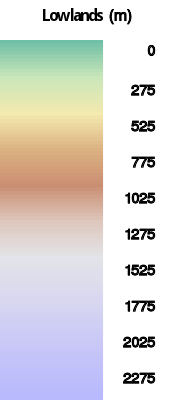
\includegraphics[angle=0,width=3.0cm,keepaspectratio='true']{figures/ramp-terrain-flatlands.png}&
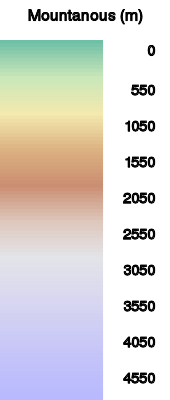
\includegraphics[angle=0,width=3.0cm,keepaspectratio='true']{figures/ramp-terrain-mountanous.png}&
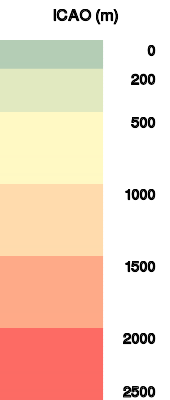
\includegraphics[angle=0,width=3.0cm,keepaspectratio='true']{figures/ramp-terrain-icao.png}&
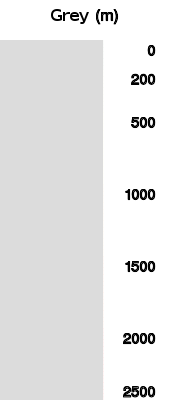
\includegraphics[angle=0,width=3.0cm,keepaspectratio='true']{figures/ramp-terrain-grey.png}
\end{longtable}

\begin{longtable}{c c c c}
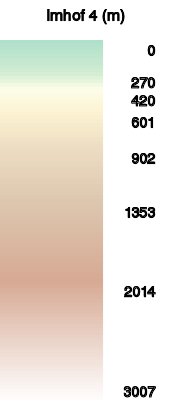
\includegraphics[angle=0,width=3.0cm,keepaspectratio='true']{figures/ramp-terrain-imhof4.png}&
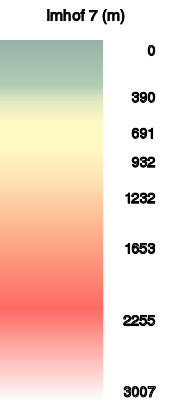
\includegraphics[angle=0,width=3.0cm,keepaspectratio='true']{figures/ramp-terrain-imhof7.png}&
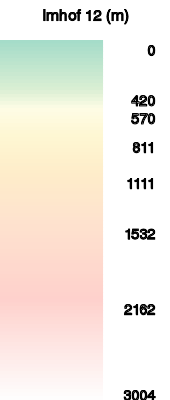
\includegraphics[angle=0,width=3.0cm,keepaspectratio='true']{figures/ramp-terrain-imhof12.png}&
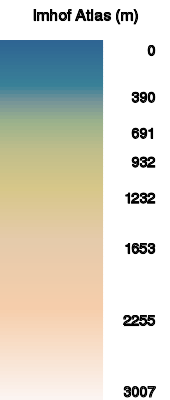
\includegraphics[angle=0,width=3.0cm,keepaspectratio='true']{figures/ramp-terrain-imhofatlas.png}
\end{longtable}


%%%%%%%%%%%%%%%%%%
\section{Map Display / Airspace}

This page is used to determine how the airspace information is
displayed and how warnings are issued.

\begin{description}
\item[Airspace display]  Controls how airspace display and warnings are filtered 
  based on altitude.  The airspace filter dialogue also allows filtering
  of display and warnings independently for each airspace class. \\
  {\bf All on}: All the airspace information is displayed at the same time. \\
  {\bf Clip}: Only airspace below a user determined altitude is shown. \\
  {\bf Auto}: Only airspace at the current altitude plus or minus a user 
    definable margin is shown.
\sketch{figures/config-airspace.png} \\
  {\bf All below}:  Like auto plus every airspace below the glider is shown.
\item[Clip altitude] For clip mode, this is the altitude below which airspace 
  is displayed.
\item[Margin]  For auto and all below airspace mode, this is the height 
  above/below which airspace is included.
\item[Warnings]  Determines whether warnings are enabled or disabled.
\item[Warning time*]  This is the time before an incursion is estimated at
  which the system will warn the pilot.
\item[Acknowledge time*]  This is the time period in which an acknowledged airspace 
  warning will not be repeated.
\item[Use black outline*]  Draws a black outline around each airspace.
\item[Airspace fill mode*]  Specifies the mode for filling the airspace area. \\
  {\bf Fill all}:  Transparently fills the airspace colour over the whole area. \\
  {\bf Fill padding}: Draws a solid outline with a half transparent border 
    around the airspace. \\
  {\bf Default}:  This selects the best performing option for your hardware. In fact 
    it favours `{\it Fill padding}' except for PPC 2000 system.
\item[Airspace transparency*]  If enabled, then airspaces are filled transparently.
\end{description}

This page also has a \button{Colours} and a \button{Filter} buttons which
can be used to review or change the colours/patterns used by each
airspace class, and whether each airspace class will be filtered out
of warnings and/or display. Depending on the airspace transparency setting it is 
no longer needed to define patterns. The availability of transparency relies 
on the capabilities of the used hardware and may differ. 

\subsection*{Colours}
This function is used to determine the colours used to draw each class of
airspaces.

First select the airspace class you wish to change. Then select the colour and 
pattern you wish the selected airspace class to be drawn in.

\subsection*{Filters}
The filter function is described in Section~\ref{sec:airspace-filter}.


%%%%%%%%%%%%%%%%%%
\section{Glide Computer / Safety Factors}

This page allows the safety heights and behaviour for the alternates mode to be defined.

\begin{description}
\item[Arrival height]  The height above terrain that the glider
  should arrive at for a safe landing.
\item[Terrain height]  \label{conf:safetyterrain} The height above terrain that 
  the glider must clear during final glide. \\
See Section~\ref{sec:safety-heights} for more details on the meanings
of the safety heights. \\
\item[Alternates mode]  \label{conf:alternatesmode} Determines sorting of alternates 
  in the alternates dialogue. \\
  {\bf Simple}: The alternates will only be sorted by arrival height. 
    The first waypoint in the list is therefore the most reachable waypoint. \\
  {\bf Task}: The sorting will also take the current task direction into account, 
    such that the sort order is according to minimum extra distance travelled to 
    the respective field and onwards to the task. \\
  {\bf Home}: The sorting will try to find landing options in the current direction 
    to the configured home waypoint.  Similar to `task' but with 
    the home field as the desired destination.
\item[Polar degradation*]  A permanent polar degradation. 0\% means no degradation, 
  50\% indicates the glider's sink rate is doubled.
\item[Safety MC*]  When safety MC is enabled, this MacCready setting is used for reach 
  calculations, task abort, alternates and for determining arrival altitude at airfields.\label{conf:safetyMC} 
\item[STF risk factor*] 
  The STF risk factor reduces the MacCready setting used to calculate
  speed to fly as the glider gets low, in order to compensate for
  risk.  Set to 0.0 for no compensation, 1.0 scales MC linearly with
\sketch{figures/config-safety.png}
  height (with reference to height of the maximum climb). If considered, 0.3 is recommended.  
  See Section~\ref{sec:safety-factor} for more details.
\end{description}


%%%%%%%%%%%%%%%%%%
\section{Glide Computer / Glide Computer}\label{sec:final-glide}\label{conf:final-glide}	

This page allows glide computer algorithms to be configured.

\begin{description}
\item[Auto MC mode]  This option defines which auto MacCready algorithm is used.
  For more details see Section~\ref{sec:auto-maccready}. \\
  {\bf Final glide}: Final glide adjusts MC for fastest arrival.
\sketch{figures/config-glidecomputer.png} \\
  {\bf Trending average climb}: Sets MC to the trending average climb rate based 
  on all climbs. \\
  {\bf Both}: Uses trending average during task, then fastest arrival when in final 
  glide mode.
\item[Block speed to fly*]  If enabled, the command speed in cruise
  is set to the MacCready speed to fly in no vertical air-mass movement.
  If disabled, the command speed in cruise is set to the dolphin speed to fly,
  equivalent to the MacCready speed with vertical air-mass movement.
\item[Nav. by baro altitude*]  When enabled and if connected to a barometric
  altimeter, barometric altitude is used for all navigation functions. Otherwise
  GPS altitude is used.
\item[Flap forces cruise*]
  When this option is enabled, causes the flap switches in Vega to
  force cruise mode when the flap is not positive. This means that
  when departing a thermal, switching to neutral or negative flap will
  immediately switch XCSoar's mode to cruise mode.
  Similarly, for Borgelt B50 systems, the speed command switch forces
  XCSoar's climb or cruise mode.
\item[GR Average period*]  Average efficiency is always calculated in real-time. 
  Here you can decide on how many seconds of flight this calculation must be done. 
  The real distance covered second by second in this period is divided by the final 
  difference of altitude.  So if for example you go and return back to the same point 
  after 2 minutes, and you have set 2 minutes as period, average GR will consider the 
  total distance covered in those two minutes, and not the distance between your 
  position 2 minutes before and your current position, that in this case could be 
  almost zero! Normally for gliders a good value is 90-120 seconds, and for paragliders 
  15 seconds. Lower values will give as a result pretty much the same as GR Instant, 
  while higher values will look like GR Cruise. Other commercial instruments and 
  software use 2 minutes.
\item[Predict wind drift*]  \label{conf:predict-drift}Account for wind drift for the predicted circling 
  duration. This reduces the arrival height for legs with head wind (on by default).
\end{description}


%%%%%%%%%%%%%%%%%%
\section{Glide Computer / Wind} \label{sec:wind}

This page sets the base for wind computations.

\begin{description}
\item[Auto wind]  \label{conf:autowind} This allows switching on or off the
  automatic wind algorithm. \\
  {\bf Manual}: When the algorithm is switched off, the pilot is responsible for
  setting the wind estimate. \\
  {\bf Circling}: Circling mode requires only a GPS source. \\
  {\bf ZigZag}: ZigZag requires an intelligent vario with airspeed output. \\
  {\bf Both}:  Uses Circling and ZigZag.
\item[Prefere external wind]  If enabled, the wind vector received from external
  devices overrides XCSoar's internal wind calculation.
\end{description}


%%%%%%%%%%%%%%%%%%
\section{Glide Computer / Route}

This page allows control over glide reach calculations and route
optimisations.

\begin{description}
\item[Route mode]  \label{conf:routemode} This controls which types
  of obstacles are used in route planning. Please have a look at Section~\ref{sec:route} 
  for a detailed description.
\item[Route climb*]  \label{conf:routeclimb} When enabled and MC is positive, route 
  planning allows climbs between the aircraft location and destination.
\item[Route ceiling*]  \label{conf:routeceiling} When enabled, route planning climbs 
  are limited to ceiling defined by greater of current aircraft altitude plus 
  500 m and the thermal ceiling.  If disabled, climbs are unlimited.
\\
\item[Reach mode]  \label{conf:turningreach} How calculations are performed of 
  the reach of the glider with respect to terrain. \\
  {\bf Off}: Reach calculations disabled. \\
  {\bf Straight}: The reach is from straight line paths from the glider. \\
  {\bf Turning}: The reach is calculated allowing turns around terrain obstacles.
\item[Reach display]  \label{conf:gliderange} This determines whether the
glide reach is drawn as a line resp.\ a shade on the map area.
\item[Reach polar*]  \label{conf:reachpolar} This determines the glide performance 
  used in reach, landable arrival, abort and alternate calculations. \\
  {\bf Task}: Uses task MacCready value; \\
  {\bf Safety MC}: Uses safety MacCready value.
\end{description}


%%%%%%%%%%%%%%%%%%
\section{Gauges / FLARM, Other} \label{sec:flarmandother-gauge}

\begin{description}
\item[FLARM radar]  \label{conf:flarmdisplay} This enables the display of the FLARM 
  radar gauge. The track bearing of the target relative to the track bearing of the 
  aircraft is displayed as an arrow head, and a triangle pointing up or down shows 
\sketch{figures/flarmrose.png}
  the relative altitude of the target relative to you.
\\
\item[Auto close FLARM*]  This will close the FLARM radar view when all FLARM 
  traffic has gone.
\item[Thermal assistant] \label{conf:thermalassistant} Enables the display of the
  ThermalAssistant gauge.
\item[Thermal band] \label{conf:thermalband} Enables the display of the
  thermal profile (climb band) overlay on the map.
\item[Final glide bar MC0*]  If set to ON the final glide bar will show a second arrow 
  indicating the required altitude to reach the final waypoint at MC zero.
\end{description}
In all FLARM environment, the colour of the target indicates the threat level.


%%%%%%%%%%
\section{Gauges / Vario}\label{sec:vario-gauge}

This page bundles all details to the vario-gauge and is entirely classified as expert setup.

\begin{description}
\item[Speed arrows*]  \label{conf:variogauge} Whether to show speed command 
  arrows on the vario gauge.
  When shown, in cruise mode, arrows point up to command slow down; arrows point down 
  to command speed up.
\item[Show average*]  Whether to show the average climb rate.  In cruise mode, this 
  switches to showing the average net airmass rate.
\item[Show MacCready*]  Whether to show the MacCready setting.
\item[Show bugs*]  Whether to show the bugs percentage.
\item[Show ballast*]  Whether to show the ballast percentage.
\item[Show gross*]  Whether to show the gross vario value.
\item[Averager needle*]  If true, the vario gauge will display a hollow averager
  needle. During cruise, this needle displays the average net value. During circling, 
  this needle displays the average gross value.
\end{description}

%%%%%%%%%%
\section{Gauges / Audio Vario}\label{sec:audiovario-gauge}

This page bundles all details to the audio vario-gauge. \label{conf:audiovariogauge}

\begin{description}
\item[Audio Vario]  Enable/Disable the audio variometer.
\item[Volume]  Set the volume of the variometer sounds.
\item[Enable Deadband]  Enable/Disable the mute for audio output when the current lift is in a certain range around zero.
\item[Min. Frequency*]  The tone frequency that is played at maximum sink rate.
\item[Zero Frequency*]  The tone frequency that is played at zero climb rate.
\item[Max. Frequency*]  The tone frequency that is played at maximum climb rate.
\item[Deadband min. lift*]  If the deadband feature is enabled the vario will play sounds when the climb rate is below this threshold.
\item[Deadband max. lift*]  If the deadband feature is enabled the vario will play sounds when the climb rate is above this threshold.
\end{description}


%%%%%%%%%%%%%%%%%%
\section{Task Defaults / Task Rules}

Task rules may be defined to limit valid starts according to competition
rules. \label{conf:taskrules}

\begin{description}
\item[Start max. speed*]  Maximum speed allowed in start observation zone.  Set 
  to 0 for no limit.
\item[Start max. speed margin*] Maximum speed above maximum start speed to tolerate. 
  Set to 0 for no tolerance.
\item[Start max. height*]  Maximum height above ground while starting the task. 
  Set to 0 for no limit.
\item[Start max. height margin*]  Maximum height above maximum start height to 
  tolerate.  Set to 0 for no tolerance.
\item[Start height ref.*]  Reference used for start max. height rule. \\
  {\bf MSL}: Reference is altitude above mean sea level. \\
  {\bf AGL}: Reference is the height above the start point.
\item[Finish min. height*]  Minimum height based on finish height reference 
  (AGL or MSL) while finishing the task.  Set to 0 for no limit.
\item[Finish height ref.*]  Reference used for finish min. height rule, 
  correspondingly to the start rule height reference.
\item[On-Line Contest]  Determines the rules used to optimize On-Line Contest 
  paths.  The implementation  conforms to the official release 2010, Sept. 23. \\
  {\bf OLC FAI}: Conforms to FAI triangle rule. Three turns and common start and 
  finish.  For tasks longer than
  500km, no leg less than 25\% or larger than 45\%; otherwise no leg less than 28\% 
  of total.  Finish height must not be lower than start height less 1000 meters. \\
  {\bf OLC Classic}: Up to seven points including start and finish, finish height
  must not be lower than start height less 1000 meters. \\
  {\bf OLC League}: A contest on top of the classic task optimisation, cutting
  a 2.5 hours segment over max. 3 of the turns. Finish height must not be below
  start height. \\
  {\bf OLC Plus}: A combination of Classic and FAI rules. 30\% of the FAI score
  are added to the Classic score. \\
  {\bf DMSt}: Deutsche Meisterschaft im Streckensegelflug. \\
  {\bf XContest}: \todonum{tbd.} \\
  {\bf DHV-XC}: \todonum{tbd.} \\
  {\bf SIS-AT}: \todonum{tbd.} \\
  {\bf FFVV NetCoupe}: The FFVV NetCoupe `{\it libre}' competition.
\item[Predict Contest]  If enabled, then the next task point is included in the 
  score calculation, assuming that you will reach it.
\end{description}


%%%%%%%%%%%%%%%%%%
\section{Task Defaults / Turnpoint Types}

This page allows to set default turnpoint types used by the task editor. All 
options are well described for the task manager in chapter~\ref{cha:tasks}.


%%%%%%%%%%%%%%%%%%
\section{Look / Language, Input}\label{sec:interface}

This page allows to customise the way the user controls and interacts with
XCSoar.

\begin{description}
\item[Auto Blank*]  This determines whether to blank the display after a long
  period of inactivity when operating on internal battery power (visible for some mobile 
  devices only).
\item[Events*]  The Input Events file defines the menu system and how XCSoar
  responds to button presses and events from external devices.
\item[Language]  The language options selects translations for English texts to
  other languages.  Select {\bf English} for a native interface, {\bf Automatic}
  to localise XCSoar according to the system settings; or you may select one of 
  the two character language short cuts directly.
\item[Status message*]  The status message file can be used to define sounds to 
  be played when certain events occur, and how long various status messages will 
  appear on screen.
\item[Menu timeout*]  This determines how long menus will appear on screen if the user
  does not make any button presses or interacts with the computer.
\item[Text Input Style*]  Determines which style for text entries is used. 
  See Section~\ref{sec:textentry} for further information on textual input. \\
  {\bf HighScore Style}: For entering text you have to change the underlined 
  character to the relevant letter. \\
  {\bf Keyboard}: Uses the on-screen keyboard for entering text. \\
  {\bf Default}: Uses the default input style for your platform.
\item[Haptic feedback*]  (Android devices only) Let you switch on or off the `{\it brrt}' 
  when the device accepts your finger press as valid input on the touch-screen.
\end{description}

Press the \button{Fonts} button to adjust the fonts XCSoar uses.

\subsection*{Font Configuration}

This page enables customisation of fonts in various fields of the program.

\sketch{figures/config-fonts.png}

Once the customisation is enabled, the \button{Edit} buttons allow to change 
some parameters (font face, height, bold and italic) of the chosen font.

If customisation is disabled, default fonts will be used.


%%%%%%%%%%%%%%%%%%
\section{Look / Screen Layout}\label{sec:interface-appearance}
\label{conf:interface-appearance}

This page once more details the appearance of the graphical user interface of XCSoar.

\begin{description}
\item[InfoBox geometry]  A list of possible InfoBox layouts. Do some trials to find the 
  best for your screen size. The preceding number refer to the total number of 
  InfoBoxes of this geometry.
\item[FLARM display*]  \label{conf:flarmradar-place}
  In case you enabled the FLARM display this is to configure the
  place on the screen, where the tiny radar window appears. As a default an `Auto' setup 
  is possible, which means that the radar window will overlay the InfoBoxes, and not the map
  part of the screen.
\item[Tab dialogue style]  Determines whether tabbed dialogues use text or icons.
\item[Message display*]  Defines the alignment of the status message box, either 
  {\bf Center} or in the {\bf TopLeft} corner.
\item[Dialogue size*]  Determines the display size of dialogues.
\item[Inverse InfoBoxes*]  If {\bf On}, the InfoBoxes are white on black, otherwise 
  black on white.
\item[Colour InfoBoxes*]  If {\bf On}, certain InfoBoxes will have coloured text. For 
  example, the active waypoint InfoBox will turn blue when the glider is above final 
  glide.
\item[InfoBox border*]  Two styles for InfoBox borders are available. \\
  {\bf Box}: Draws boxes around each InfoBox. \\
  {\bf Tab}: Draws a tab at the top of the InfoBox across the 
  title. \\
\end{description}


%%%%%%%%%%%%%%%%%%
\section{Look / InfoBox Pages (or just Pages)}\label{conf:screenpages}

This page allows the definition of the screen page ensemble. A typical setup 
will contain three pages, the expert can pile up to eight possible pages.

A page is more or less a composition of map and InfoBox set. There are five 
predefined pages for circling, cruise, final glide, a map only page and a 
page with automatic InfoBox set activation depending on your flight mode.

Additionally you can choose from up to five more pages that are composed from map 
and your custom InfoBox sets.  

\begin{description}
\item[Page 1..3]  Select what you feel is appropriate for you to appear on page 1,2,3 etc. 
  Selecting "- - -" will let the page inactive.
\item[Page 4..8*]  Experts can configure up to eight pages in the already 
  described manner.
\end{description}


%%%%%%%%%%
\section{Look / InfoBox Modes (or InfoBox Sets)}\label{sec:infobox_sets}
\label{conf:infobox_sets}

This page shows and let you customise the available InfoBox sets.

\begin{description}
\item[Circling, Cruise, ...]  There are three predefined InfoBox sets (Circling, Cruise, Final Glide). 
  Additionally you can define up to five more InfoBox sets and name them as you want.   
  By default they are named AUX-1, AUX-2, and so on. \\
  Selecting one of the sets starts a dialogue which provides all means to name and 
  compose an InfoBox set up to your needs.

\item[Use final glide mode]  Controls whether the "final glide" InfoBox mode should be used on "auto" pages.
\end{description}

\subsection*{InfoBox Set Customisation}

\begin{description}
\item[Name]  Sets the name of the currently customized InfoBox set. The 
  button starts the text input dialogue of XCSoar.
\item[InfoBox]  The number identifying the current box.
\item[Content]  Select the information you want to see at the current box.
\end{description}

The right side of the dialogue always gives the overview on the composed set. 
When composing at the PC you can use the mouse to select the individual boxes 
right from the overview.

See Section~\ref{cha:infobox} for a description of the InfoBox types and their meanings.

To change a set press on one of the InfoBoxes labeled with it's current content.
The InfoBoxes are numbered; the location of the InfoBoxes depends on the screen layout.  
The tables below shows the InfoBox enumeration scheme for the 
landscape and portait screen layout.

\begin{multicols}{2}
\begin{tabular}{|c|c|}
\hline
1 & 7 \\
\hline
2 & 8 \\
\hline
3 & 9 \\
\hline
4 & 10 \\
\hline
5 & 11 \\
\hline
6 & 12 \\
\hline
\end{tabular}

\begin{tabular}{|c|c|c|c|}
\hline
1 & 2 & 3 & 4 \\
\hline
\hline
5 & 6 & 7 & 8 \\
\hline
\end{tabular}
\end{multicols}

%%%%%%%%%%%%%%%%%%
\section{Setup / Devices} \label{conf:comdevices}

The Devices page is used to specify the ports used to communicate with
the GPS and other serial devices. The default settings are COM1 and
4800 bits per second.  When connected to the Vega intelligent
variometer, the settings should be COM1 and 38400.

Four devices can be configured (device A through D). One, for
example, can be connected to a GPS and another to a
second device such as a variometer.  If there is no further device, 
set the unused ports to `Disabled'.  XCSoar will then ignore those ports.
\sketch{figures/config-devices.png}

COM ports 0 to 10 may be used, including a TCP/IP connection.  
Which COM port is appropriate for you
depends on what brand of PDA you use, and the communications medium
(serial cable, Bluetooth, virtual COM port, SD card or CF based GPS,
internal GPS).  Detailing the various options for different devices is
beyond the scope of this document.  If you have trouble identifying
which COM port to set, please refer to the XCSoar website and mailing
lists.

\begin{description}
\item[Port]  This setting maps an existing interface (port) of your 
  glide computer to one of the available slots A to D.
\item[Baudrate]  Set this to the communication speed of the connected device.
\item[TCP Port]  This setting is useful to e.g. connect to the Condor flight
  simulator and do some XCSoar training in winter time.
\item[Bulk baud rate]  The baud rate used for bulk transfers, such 
  as task declaration or flight download. The item is visible for those 
  devices that support the feature.
\item[Driver]  The specific type of device can be selected from a list in order
  to enable support for devices with proprietary protocols or special
  functions.
\item[Sync. from device*]  This option lets you configure if XCSoar should use settings 
  like the MacCready value, bugs and ballast from the device.
\item[Sync. to device*]  This option lets you configure if XCSoar should send settings 
  like the MacCready value, bugs and ballast to the device.
\item[Ignore checksum*] If your GPS device outputs invalid NMEA checksums, this 
  will allow it's data to be used anyway.
\end{description}


%%%%%%%%%%%%%%%%%%
\section{Setup / Polar}

This page allows the glide polar to be defined. For a large variety of glider types 
XCSoar provides a predefined glide polar, they could be modified if needed, or 
you can load your own polar from a file. 
The file format is based on the WinPilot polar file format (see section~\ref{sec:glide-polar}).

\label{conf:polar} To configure the glide computer to the performance of a glider 
type start with the selection of a type from the \button{List}. 
Choose \button{Import} when you want to load an external polar file.
Customise the three V/W points defining the parable curve and the reference 
weight to your needs. 
\tip Be aware that namely those four items are of crucial importance 
for every glide performance relevant computation of XCSoar.   
\button{Export} your efforts to a file is always a good idea.

\begin{description}
\item[Polar V/W]  Three pairs of corresponding horizontal and vertical speed of the glider. 
  A good choice for the point triplet is one at the top most area of the polar, the second at a 
  still very curved area and the third far out where the curvature seems to disappear.
\item[Reference mass]  Reference weight at which the given polar is valid.
\item[Dry mass]  The complete weight of the rigged glider including the pilots weight except the 
  loaded water ballast. 
  In the absence of a configurable pilot weight XCSoar expect you to include your own weight 
  to the dry mass.
\item[Wing area]  Optional specification of the wing area of the glider type.
\item[V rough air] Optional the maximum manoeuvring speed can 
  be entered on this page to prevent the glide computer from commanding 
  unrealistic cruise speeds.
\item[Handicap]  The handicap factor used for the On-Line Contest scoring.
\item[Max. ballast]  Optional the amount of water ballast XCSoar refers to as 100\% ballast.
  Set to zero if it does not apply.
\item[Dump time]  The time in seconds needed for dumping full ballast.
\end{description}


%%%%%%%%%%%%%%%%%%
\section{Setup / Logger} \label{conf:logger}

The internal software logger has adjustable time steps, separate for
cruise and circling modes.  
Typically the circling time step is set to a smaller value
than cruise in order to give good quality flight logs for replay
purposes.

\begin{description}
\item[Time step cruise*]  This is the time interval between logged points when 
  not circling. 
\item[Time step circling*]  This is the time interval between logged points when 
  circling. 
\item[Auto logger*]  Enables the automatic starting and stopping of the logger
  on takeoff and landing respectively. Disable when flying paragliders to prevent 
  the low ground speeds from triggering the automatic logger.
\item[NMEA logger*]  Enable the NMEA logger on startup? If this option is disabled, 
  the NMEA logger can still be started manually.
\item[Log book*]  Logs each start and landing.
\end{description}


%%%%%%%%%%%%%%%%%%
\section{Setup / Logger info} \label{conf:logger_info}

This page allows you to set the pilot and aircraft details used for
annotating XCSoar's IGC logger.  

\begin{description}
\item[Pilot name]  This is the pilot name used in the internal software logger 
  declaration.
\item[Aircraft type]  This is the aircraft type used in the internal software 
  logger declaration.
\item[Aircraft reg.]  This is the aircraft registration used in the internal 
  software logger declaration.
\item[Competition ID]  This is the aircraft competition ID.
\item[Logger ID]  This is the logger registration.
\end{description}


%%%%%%%%%%%%%%%%%%
\section{Setup / Units}

This page allows you to set the units preferences used in all
displays, InfoBoxes, dialogues and input fields.  
For most users hopefully one of the presets will match the needs.  The presets 
include unit sets for {\bf American}, {\bf Australian}, {\bf British}, 
and {\bf European}.

Separate selections are available for all items. Once you changed a given preset it 
will be referenced as `Custom' set and will also be stored in your profile.

\begin{description}
\item[Aircraft/Wind speed*]  Units used for airspeed and ground speed: mph, 
  knots, km/h. A separate unit is available for task speeds.
\item[Distance*]  Units used for horizontal distances e.g. range to waypoint, 
  distance to go: sm, nm, km.
\item[Lift*]  Units used for vertical speeds (variometer): knots, m/s, ft/min.
\item[Altitude*] Units used for altitude and heights: foot/meter.
\item[Temperature*]  Units used for temperature: \degree C, \degree F.
\item[Task speed*] Units used for task speed: mph, knots, km/h.
\item[Pressure*]  Units used for pressures: hPa, mb, inHg.
\item[Lat./Lon.*]  Units, or better formats used for latitude and longitude. 
  Supported are several `degree/minutes/seconds' formats, respectively 
  their decimal fraction, and the  UTM WGS 84 format.
\end{description}


%%%%%%%%%%%%%%%%%%
\section{Setup / Time}

Set the local time offset with respect to UTC.

\begin{description}
\item[UTC offset]  The field allows the UTC local time offset to be specified.
\item[Local time]  The local time is displayed below in order to make it easier to verify
  the correct offset has been entered.  Offsets to the half-hour may be set.
\item[Use GPS time*] This option, if enabled sets the clock of the computer to 
  the GPS time once a fix is set. This is only necessary if your computer does 
  not have a real-time clock with battery backup or your computer 
  frequently runs out of battery power or otherwise loses time.
\end{description}


%%%%%%%%%%%%%%%%%%
\section{Setup / Tracking}

`{\it Live}'-Tracking means using a GPS to determine your position and a mobile 
network to send this position in real-time to a server, other people can see 
your excact position and track presented in a map just in time.
The tracking option needs the capability to connect to mobile networking as offered by 
your glide computer.

Currently there are two tracking protocolls implemented. `{\em SkyLines}' as a spin 
off project from XCSoar itself; for details on this service have a look at 
\url{http://skylines.xcsoar.org}. 
And also the `{\em LiveTrack24}' protocoll used e.g. by the tracking 
portal on \url{http://www.livetrack24.com}.  
Please consult the web pages of the service provider listed under `Server' 
for details on this setup.

\begin{description}
\item[SkyLines]  Switch this {\bf On} to enable the live stream of 
  your position to `{\em SkyLines}'.
\item[Tracking Interval]  The time interval for which one position is send to 
  the tracking service. `{\em SkyLines}' implements a very lean protocol, so that even
  a 30 sec. interval does not exhaust a plain GPRS connection (ca. 12kbit/sec). 
\item[Key]  Create a key on the page \url{http://skylines.xcsoar.org/tracking/info} 
  and enter it here, to identify your positions at the tracking service.
\\
\item[LiveTrack24]  Switch this {\bf On} to enable the live stream of 
  your position to `{\em LiveTrack24}'.
\item[Tracking Interval]  The time interval for which one position is send to 
  the tracking service.
\item[Vehicle Type]  Type of vehicle used.
\item[Server]  The service's web address to stream your position to. There is currently 
  a choice of some predefined.
\item[Username]  If you created an account you can enter those credentials here. 
  Otherwise the track will be logged as `{\it guest}' and thus be anonymous.  
\item[Password]  The password to your tracking account.
\end{description}

